\documentclass{fancyslides} 
\usepackage[utf8]{inputenc}
\usepackage{times}

\usepackage{graphicx}
\usepackage{caption}
\usepackage{subcaption}


\graphicspath{{img/}}

%%% Beamer settings (do not change)
\usetheme{default} 
\setbeamertemplate{navigation symbols}{} %no navigation symbols
\setbeamercolor{structure}{fg=\yourowntexcol} 
\setbeamercolor{normal text}{fg=\yourowntexcol} 



%%%%%%%%%%%%%%%%%%%%%%%%%
%%% CUSTOMISATIONS %%%%%%
%%%%%%%%%%%%%%%%%%%%%%%%%


%%%% SLIDE ELEMENTS
\newcommand{\structureopacity}{0.75} %opacity for the structure elements (boxes and dots)
\newcommand{\strcolor}{black} %elements colour (predefined blue; orange; green)

%%%% TEXT COLOUR
\newcommand{\yourowntexcol}{white}


%%%%%%%%%%%%%%%%%%%%%%%%%
%%% TITLE SLIDE DATA %%%%
%%%%%%%%%%%%%%%%%%%%%%%%%
\fbckg{abstract-data}
\newcommand{\titlephrase}{On-Line Analytical Processing}
\newcommand{\name}{Javier Bonet \\ Joel Catacora \\}
\newcommand{\affil}{Base de datos avanzada}
\newcommand{\email}{22 de abril del 2015}


\begin{document}


\startingslide %this generates titlepage from the data above

\fbckg{white}
\begin{frame}
\pointedsl{{\LARGE ¿Qué es OLAP?}}
\end{frame}


\fbckg{white}
\begin{frame}
\misc
{
El \textbf{procesamiento analítico en línea} (OLAP) es una solución utilizada en el campo de la inteligencia de negocios, cuyo objetivo es permitir la consulta de grandes cantidades de datos de forma eficiente y sencilla.
}
\end{frame}

\fbckg{white}
\begin{frame}
\misc
{
El concepto OLAP puede definirse mediante 5 palabras: Análisis Rápido de Información Compartida Multidimensional, (Fast Analysis of Shared Multidimensional Information, o FASMI).
}
\end{frame}

\fbckg{white}
\begin{frame}
\misc
{
\begin{itemize}
  \item \textbf{Rápida}: el sistema está dirigido a proporcionar la mayoría de las respuestas a los usuarios en pocos segundos.
  \item \textbf{Análisis}: el sistema puede hacer frente a cualquier lógica de negocio y análisis estadístico que sea relevante para el usuario, en forma relativamente sencilla.
  \item \textbf{Compartida}: significa que el sistema implementa todos los requisitos de seguridad de la confidencialidad.
  \item \textbf{Multidimensionalidad}: el sistema debe proveer una vista conceptual multidimensional de los datos.
  \item \textbf{Información}: se refiere a todos los datos y la información derivada, que sea relevante para la aplicación.
\end{itemize}
}
\end{frame}



\fbckg{white}
\begin{frame}
\pointedsl{{\LARGE Características}}
\end{frame}


\fbckg{white}
\begin{frame}
\itemized{
\item \textbf{Soportar cálculos complejos}
}
\end{frame}

\fbckg{white}
\begin{frame}
\itemized{
\item \textbf{Soportar cálculos complejos}
\item \textbf{Rapidez de respuesta}
}
\end{frame}

\fbckg{white}
\begin{frame}
\itemized{
\item \textbf{Soportar cálculos complejos}
\item \textbf{Rapidez de respuesta}
\item \textbf{Inteligencia respecto del tiempo}
}
\end{frame}


\fbckg{white}
\begin{frame}
\pointedsl{{\LARGE Reglas de Codd}}
\end{frame}

\fbckg{white}
\begin{frame}
\itemized{
\item \textbf{Visión multidimensional}
}
\end{frame}

\fbckg{white}
\begin{frame}
\itemized{
\item \textbf{Visión multidimensional}
\item \textbf{Manipulación intuitiva de los datos}
}
\end{frame}

\fbckg{white}
\begin{frame}
\itemized{
\item \textbf{Visión multidimensional}
\item \textbf{Manipulación intuitiva de los datos}
\item \textbf{Accesibilidad}
}
\end{frame}

\fbckg{white}
\begin{frame}
\itemized{
\item \textbf{Visión multidimensional}
\item \textbf{Manipulación intuitiva de los datos}
\item \textbf{Accesibilidad}
\item \textbf{Soporte multi-usuario}
}
\end{frame}

\fbckg{white}
\begin{frame}
\itemized{
\item \textbf{Visión multidimensional}
\item \textbf{Manipulación intuitiva de los datos}
\item \textbf{Accesibilidad}
\item \textbf{Soporte multi-usuario}
\item \textbf{Información separada del origen de datos}
}
\end{frame}

\fbckg{white}
\begin{frame}
\itemized{
\item \textbf{Visión multidimensional}
\item \textbf{Manipulación intuitiva de los datos}
\item \textbf{Accesibilidad}
\item \textbf{Soporte multi-usuario}
\item \textbf{Información separada del origen de datos}
\item \textbf{Flexibilidad ante valores nulos}
}
\end{frame}

\fbckg{white}
\begin{frame}
\itemized{
\item \textbf{Visión multidimensional}
\item \textbf{Manipulación intuitiva de los datos}
\item \textbf{Accesibilidad}
\item \textbf{Soporte multi-usuario}
\item \textbf{Información separada del origen de datos}
\item \textbf{Flexibilidad ante valores nulos}
\item \textbf{Rendimiento uniforme}
}
\end{frame}

\fbckg{white}
\begin{frame}
\itemized{
\item \textbf{Visión multidimensional}
\item \textbf{Manipulación intuitiva de los datos}
\item \textbf{Accesibilidad}
\item \textbf{Soporte multi-usuario}
\item \textbf{Información separada del origen de datos}
\item \textbf{Flexibilidad ante valores nulos}
\item \textbf{Rendimiento uniforme}
\item \textbf{Dimensiones y niveles de agregación ilimitados}
}
\end{frame}

\fbckg{white}
\begin{frame}
\pointedsl{\LARGE{Jerarquías}}
\end{frame}

\fbckg{white}
\begin{frame}
\misc
{
  Las \textbf{jerarquías} se utilizan para especificar en menor o mayor detalle los datos contenidos en la dimensión. Las jerarquías son de mucha utilidad a la hora de calcular valores "agregados"\\ \ \\ \ \\

  \underline{Ejemplos:}
  \begin{center}
  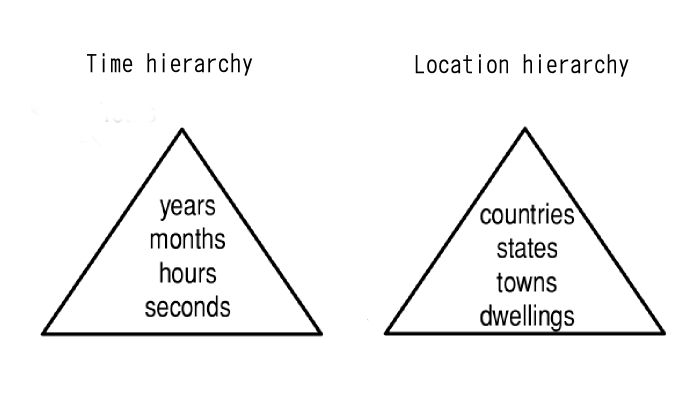
\includegraphics[scale=0.3]{jerarquias}
  \end{center}
}
\end{frame}


\fbckg{white}
\begin{frame}
\pointedsl{\LARGE{Agregaciones}}
\end{frame}

\fbckg{white}
\begin{frame}
\misc
{
Los \textbf{agregados} se utilizan en los modelos dimensionales del Data Warehouse para producir efectos positivos sobre el tiempo que toma una consulta sobre grandes conjuntos de datos. El uso más común de los agregados es tomar una dimensión y cambiar su granularidad.
Al cambiar la granularidad de la dimensión, la tabla de hechos tiene que ser parcialmente resumida para adaptarse a la nueva dimensión. Se crean así, nuevas tablas de dimensiones y tablas de hechos, que encajan en este nuevo nivel de granularidad.
}
\end{frame}

\fbckg{white}
\begin{frame}
\misc
{
\begin{figure}
        \centering
        \begin{subfigure}[b]{0.5\textwidth}
                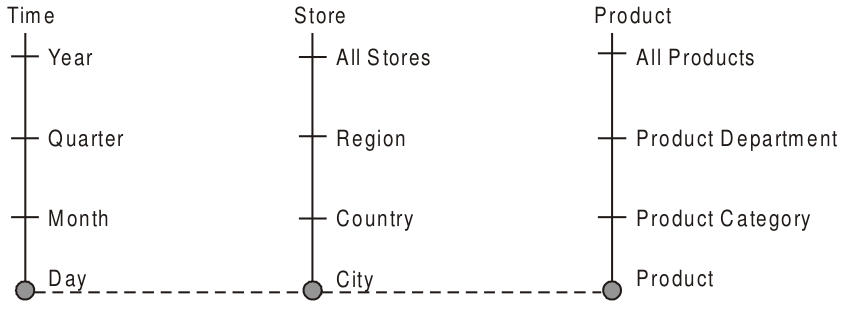
\includegraphics[width=\textwidth]{ej1_agregados}

                Esquema de nivel base que usa la parte inferior del nivel de je-rarquías dimensionales.
        \end{subfigure}%
        ~ \quad
        \begin{subfigure}[b]{0.5\textwidth}
                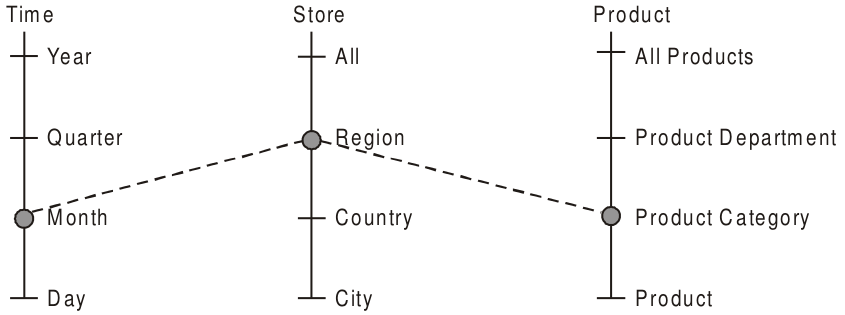
\includegraphics[width=\textwidth]{ej2_agregados}
                
                Esquema agregado, que resulta en datos de un nivel más alto en las jerarquía dimensionales.
        \end{subfigure}
\end{figure}

Los esquemas agregados proporcionan mejoras en el rendimiento debido a que tienen un número significativamente menor de registros.

}
\end{frame}


\fbckg{white}
\begin{frame}
\misc
{
\textbf{Ejemplo:}

Este esquema copo de nieve, tiene una sola tabla de echos \textit{Sales}, dos métricas (\textit{units and dollars}) y cuatro tablas de dimensiones (\textit{Product, Mfr, Customer, Time, y Customer}).

\begin{center}
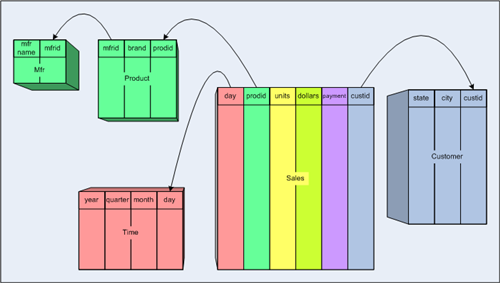
\includegraphics[scale=0.4]{aggregate_tables_1}
\end{center}
}
\end{frame}

\fbckg{white}
\begin{frame}
\misc
{
\textbf{Ejemplo:}

Creamos una tabla agregada, \textbf{Agg\_1}:
 
\begin{center}
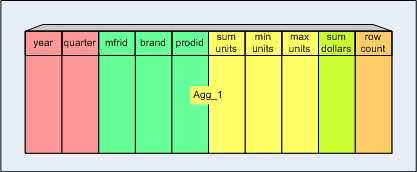
\includegraphics[scale=0.5]{aggregate_tables_2}
\end{center}
}
\end{frame}

\fbckg{white}
\begin{frame}
\misc
{Veamos como las columnas del esquema original se han combinado en la tabla \textbf{Agg\_1}:

\begin{itemize}
  \item La dimensión \textit{Time} se "colapsó" en la tabla de agregación, omitiendo las columnas \textit{month} y \textit{day}.
  \item Las dos tablas de la dimensión \textit{Product} se "colapsaron" en la tabla de agregación.
  \item La dimensión \textit{Customer} se "perdió".
  \item Para cada métrica en la tabla de hechos (\textit{units, dollars}), hay uno o más métricas en la tabla de agregación (\textit{sum units, min units, max units, sum dollars}).
  \item También hay una nueva métrica, \textit{row count}, que representa la métrica "conteo".
\end{itemize}
}
\end{frame}


\fbckg{white}
\begin{frame}
\misc
{
\textbf{Ejemplo}

Otra tabla agregada, \textbf{Agg\_2}:

\begin{center}
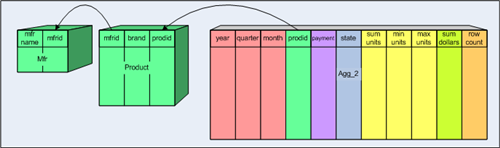
\includegraphics[scale=0.5]{aggregate_tables_3}
\end{center}

Varias dimensiones colapsaron: \textit{Time} en el nivel \textit{Quarter}; \textit{Customer} en el nivel \textit{State};
y \textit{Payment Method} a nivel \textit{Payment Method}. Pero la dimensión \textit{Product} se conservó.}
\end{frame}


\fbckg{white}
\begin{frame}
\misc
{
Tener datos agregados en el modelo dimensional hace que el entorno sea más complejo.
Para que esta complejidad adicional sea transparente al usuario, se utiliza una funcionalidad conocida como \textit{navegación de agregados},
la cual es implementada por el motor OLAP, para consultar las tablas dimensionales y de hecho, con el nivel de granularidad correcto.
}
\end{frame}

\fbckg{white}
\begin{frame}
\pointedsl{\LARGE{Hipercubo de datos}}
\end{frame}

\fbckg{white}
\begin{frame}
\misc
{
El cubo OLAP puede ser pensado como una extensión de la matriz multidimensional de una hoja de cálculo, de ahí el nombre del hipercubo. Técnicamente, el cubo de datos es una representación multidimensional de datos, junto con todos los agregados posible, es decir, los agregados que resultan mediante la selección de un subconjunto propio de las dimensiones y sumando sobre todas las dimensiones restantes.
}
\end{frame}


\fbckg{white}
\begin{frame}
\misc
{
Tomaremos como ejemplo el siguiente conjunto de datos:
\begin{center}
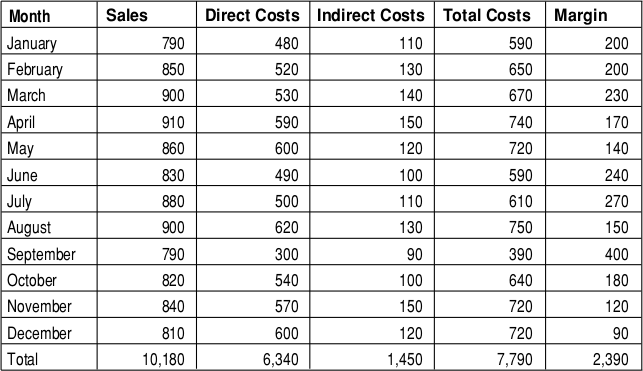
\includegraphics[scale=0.4]{cube_1}
\end{center}
}
\end{frame}


\fbckg{white}
\begin{frame}
\misc
{
\textit{Sales}, \textit{costs}, y \textit{margin} representan \textit{variables}.

Si alguien pregunta, "¿Qué estás midiendo?".

Le respondemos, "ventas, costos y márgenes".

Mientras que, los meses representan la organización de los datos.

Ante la pregunta, "¿De dónde consigue sus datos?", o "¿con qué frecuencia está haciendo mediciones?".

Responderíamos, "Estamos siguiendo las ventas mensuales."
\newline

Entonces, utilizando los conceptos dados en la charla \textit{Data Warehouse}, tenemos tres \textbf{hechos},
y dos \textbf{dimensiónes}, el \textit{tiempo}, y las \textit{variables}.
}
\end{frame}

\fbckg{white}
\begin{frame}
\misc
{
¿Qué sucede cuando añadimos una tercera dimensión llamada \textit{products} (productos)?.
Tenemos un cubo.

\begin{center}
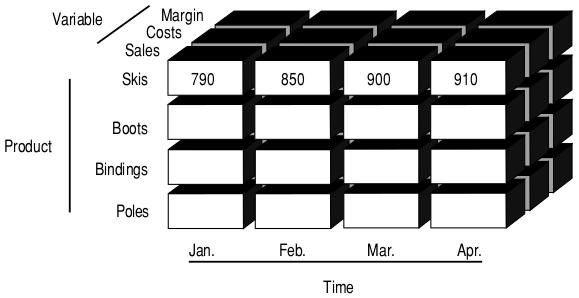
\includegraphics[scale=0.4]{cube_2}
\end{center}
}
\end{frame}

\fbckg{white}
\begin{frame}
\misc
{
El conjunto de datos tridimensionales que consiste de \textit{variables}, \textit{time}, y \textit{products}, se puede mostrar en una pantalla en términos de: fila, columna y página.

\begin{center}
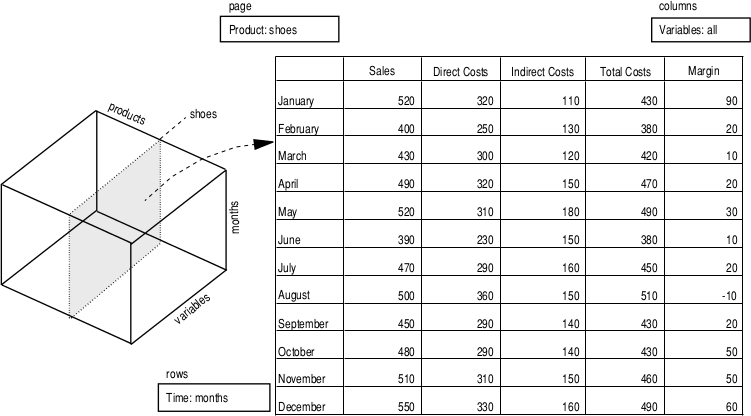
\includegraphics[scale=0.3]{cube_3}
\end{center}
}
\end{frame}


\fbckg{white}
\begin{frame}
\misc
{
¿Qué sucede si intentamos añadir una dimensión tienda (\textit{ store}) al cubo?.

Presentamos una nueva metáfora para representar datos, o eventos generadores de datos, que es capaz de reproducir cualquier número de dimensiones.

La llamamos, \textbf{estructura de tipo multidimensional} (\textit{Multidimensional Type Structures}, o MTS).

Cada dimensión está representada por una línea. Cada miembro dentro de una dimensión está representado por un intervalo, dentro del segmento correspondiente.
}
\end{frame}

\fbckg{white}
\begin{frame}
\misc
{
Siguiendo el ejemplo de tres dimensiones, hay tres líneas:

una para el \textit{tiempo}, una de los \textit{productos}, y una de las \textit{variables}.

Cualquier unión de los intervalos, de cada uno de los tres segmentos, está conectado a un evento y a un elemento del cubo.

\begin{center}
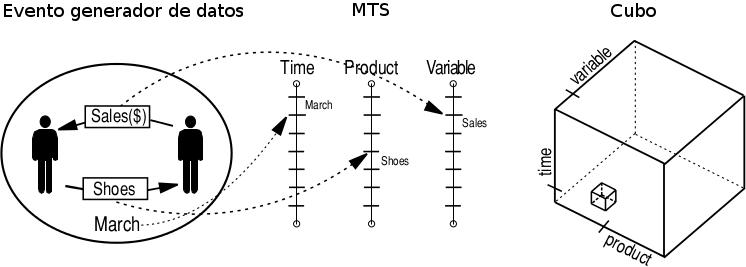
\includegraphics[scale=0.3]{cube_4}
\end{center}
}
\end{frame}

\fbckg{white}
\begin{frame}
\misc
{
Para ver los datos en la pantalla, tenemos que mappear múltiples dimensiones lógicas en dos dimensiones físicas (la pantalla).
}
\end{frame}


\fbckg{white}
\begin{frame}
\misc
{
\begin{figure}
        \centering
        \begin{subfigure}[b]{0.7\textwidth}
                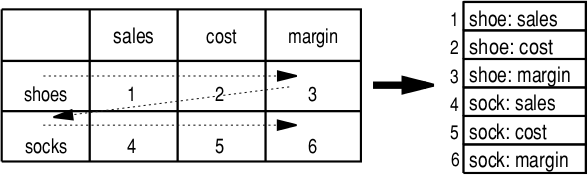
\includegraphics[width=\textwidth]{cube_5}

                Variables anidadas con productos.
        \end{subfigure}
        
        
        \ \hfil
        
        
        \begin{subfigure}[b]{0.7\textwidth}
                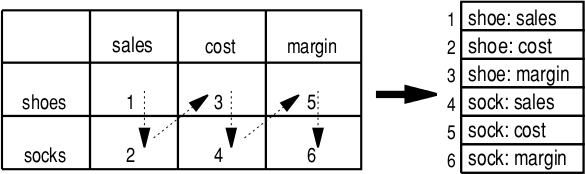
\includegraphics[width=\textwidth]{cube_6}
                
                Productos anidados con variables
        \end{subfigure}
\end{figure}
}
\end{frame}

\fbckg{white}
\begin{frame}
\misc
{
Efectos de combinar dimensiones:

{
\begin{figure}
        \centering
        \begin{subfigure}[b]{0.4\textwidth}
          $\textendash$ Cambia la forma de los datos visibles. La longi-tud de una lista unidimensional es igual al producto de las longitudes de cada una de las dos dimensiones.
          
          $\textendash$ Cambia el conjunto de vecinos que rodean cualquier punto.
        \end{subfigure}
        ~
        \begin{subfigure}[b]{0.4\textwidth}
          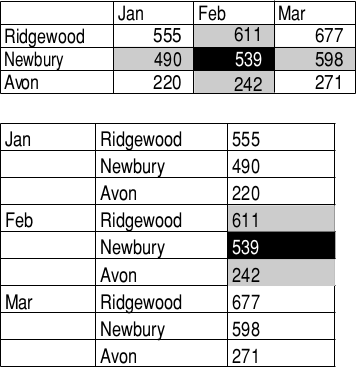
\includegraphics[width=\textwidth]{cube_7}
        \end{subfigure}
\end{figure}
}
}
\end{frame}

\fbckg{white}
\begin{frame}
\misc
{
Ahora tenemos un conjunto de datos que consiste de: \textit{products}, \textit{times}, \textit{stores}, \textit{customers}, \textit{variables}, y \textit{scenarios}.
\begin{figure}
        \centering
        \begin{subfigure}[b]{0.5\textwidth}
                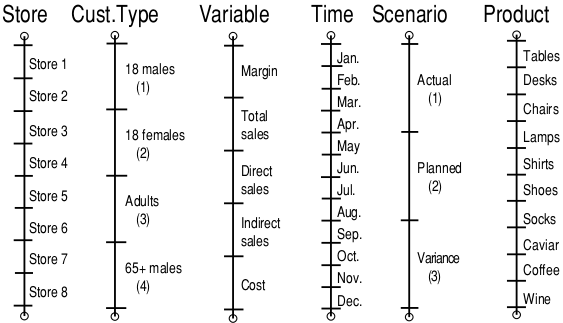
\includegraphics[width=\textwidth]{cube_8}
        \end{subfigure}%
        ~
        \begin{subfigure}[b]{0.55\textwidth}
                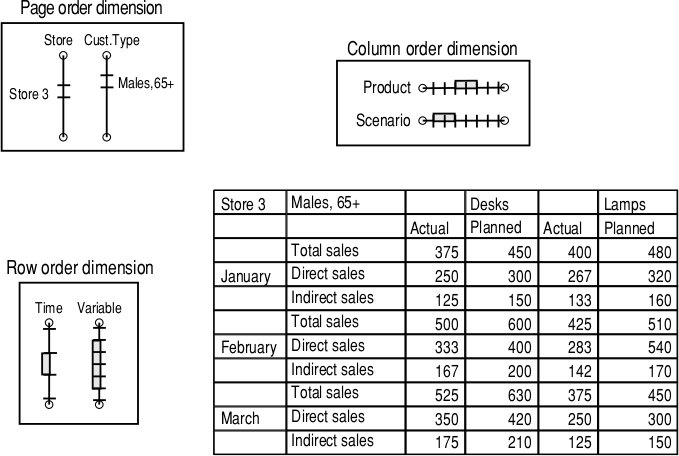
\includegraphics[width=\textwidth]{cube_9}
        \end{subfigure}
\end{figure}
}
\end{frame}

\fbckg{white}
\begin{frame}
\misc
{
La capacidad de cambiar fácilmente las vistas de los mismos datos, mediante la reconfiguración de cómo se muestran las dimensiones, es uno de los grandes beneficios
que proveen los sistemas multidimensionales, a la navegación de los usuarios finales.
Esto se debe a la separación de la estructura de datos (MTS), de su visualización (rejilla multidimensional).
}
\end{frame}


\fbckg{white}
\begin{frame}
\misc
{
Hay algunas reglas básicas que usted debe tener en cuenta en el análisis de datos multidimensionales:
\begin{itemize}
  \item Debe tratar de utilizar páginas. Esto ayuda a maximizar el grado en que todo en la pantalla es relevante.
  \item Cuando necesita anidar múltiples dimensiones a través de las filas y columnas, generalmente es mejor anidar más dimensiones a través de las columnas que a través de las filas, ya que suele haber mas espacio vertical en la pantalla, que horizontal.
  \item Antes de decidir cómo mostrar la información en la pantalla, pregúntese "¿Qué quiero mirar?", o "¿Qué estoy tratando de comparar?".
\end{itemize}
}
\end{frame}

\fbckg{white}
\begin{frame}
\misc
{ Vista clásica:
\begin{center}
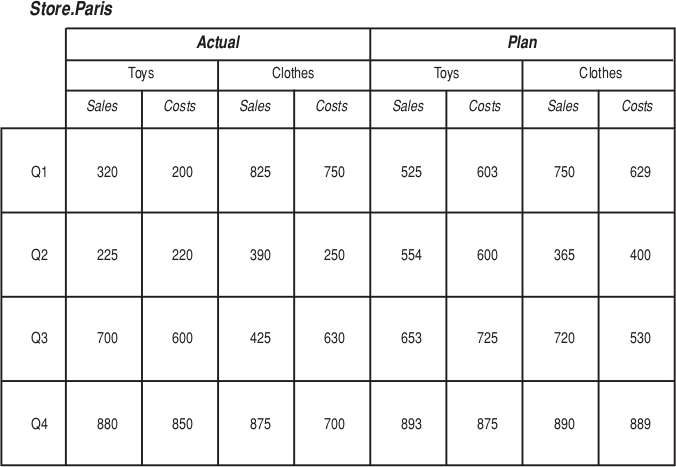
\includegraphics[scale=0.4]{cube_10}
\end{center}
}
\end{frame}


\fbckg{white}
\begin{frame}
\pointedsl{\LARGE{Operaciones}}
\end{frame}


\fbckg{white}
\begin{frame}
\misc
{
  \underline{Slice:}\\
  Consiste en obtener una rebanada del cubo que se está visualizando
}
\end{frame}

\fbckg{white}
\begin{frame}
\misc
{
  \begin{center}
  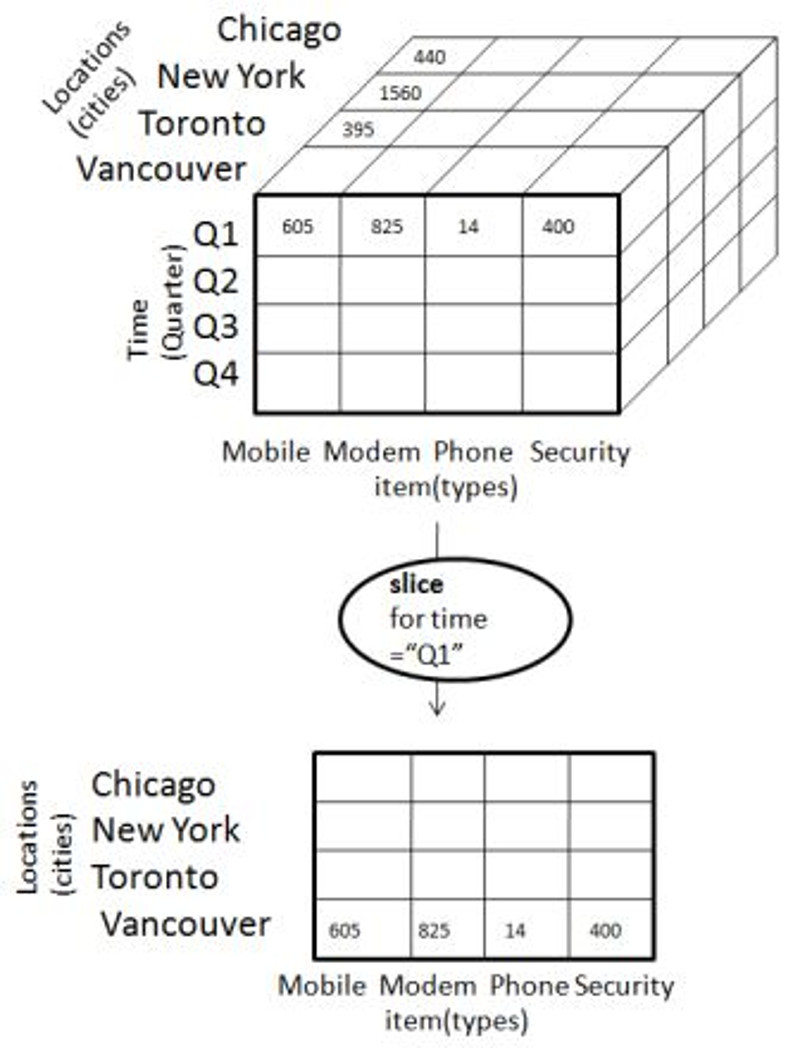
\includegraphics[scale=0.15]{slice}
  \end{center}
}
\end{frame}


\fbckg{white}
\begin{frame}
\misc
{
  \underline{Dice:}\\
  Seleccionar valores específicos para 2 o más dimensiones de las dimensiones que se visualizan
  y con esto obtener un subcubo 
}
\end{frame}

\fbckg{white}
\begin{frame}
\misc
{
  \begin{center}
  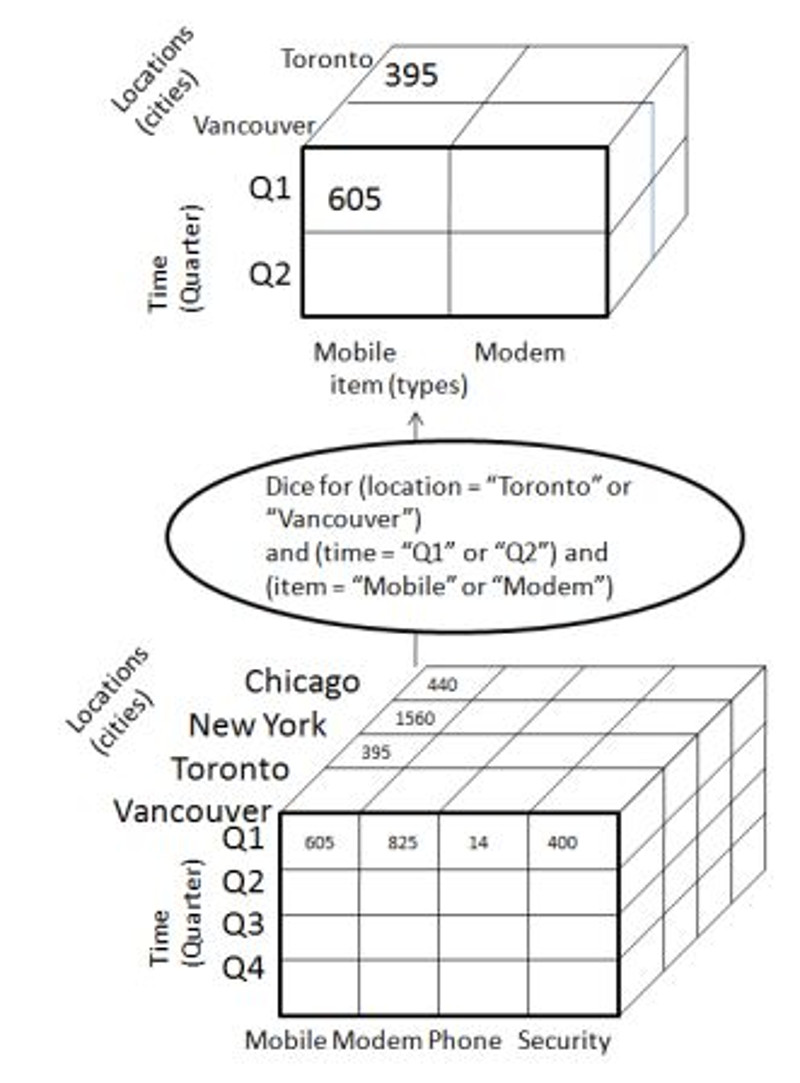
\includegraphics[scale=0.15]{dice}
  \end{center}
}
\end{frame}


\fbckg{white}
\begin{frame}
\misc
{
  \underline{Drill Down:}\\
  Al aplicar esta operación buscamos obtener un mayor nivel de detalle
}
\end{frame}

\fbckg{white}
\begin{frame}
\misc
{
  \begin{center}
  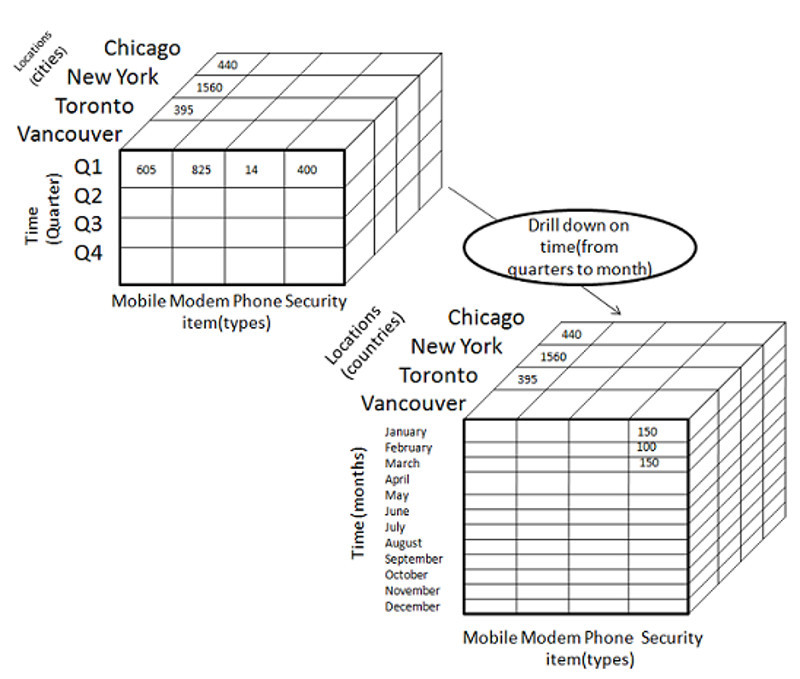
\includegraphics[scale=0.5]{drill_down}
  \end{center}
}
\end{frame}


\fbckg{white}
\begin{frame}
\misc
{
  \underline{Drill Up:}\\
  Menor nivel de detalle y, por ende, mayor nivel de sumarización
}
\end{frame}

\fbckg{white}
\begin{frame}
\misc
{
  \begin{center}
  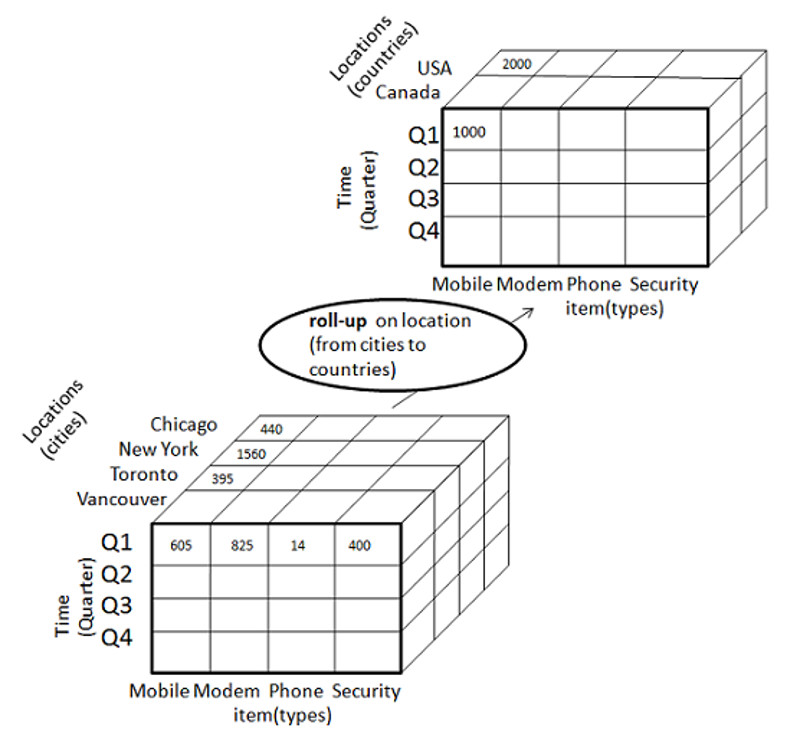
\includegraphics[scale=0.2]{drill_up}
  \end{center}
}
\end{frame}


\fbckg{white}
\begin{frame}
\misc
{
  \underline{Pivot:}\\
  Aplicando esta operacion ofrecemos al usuario una presentación alternativa de la información rotando los ejes de datos
}
\end{frame}

\fbckg{white}
\begin{frame}
\misc
{
  \begin{center}
  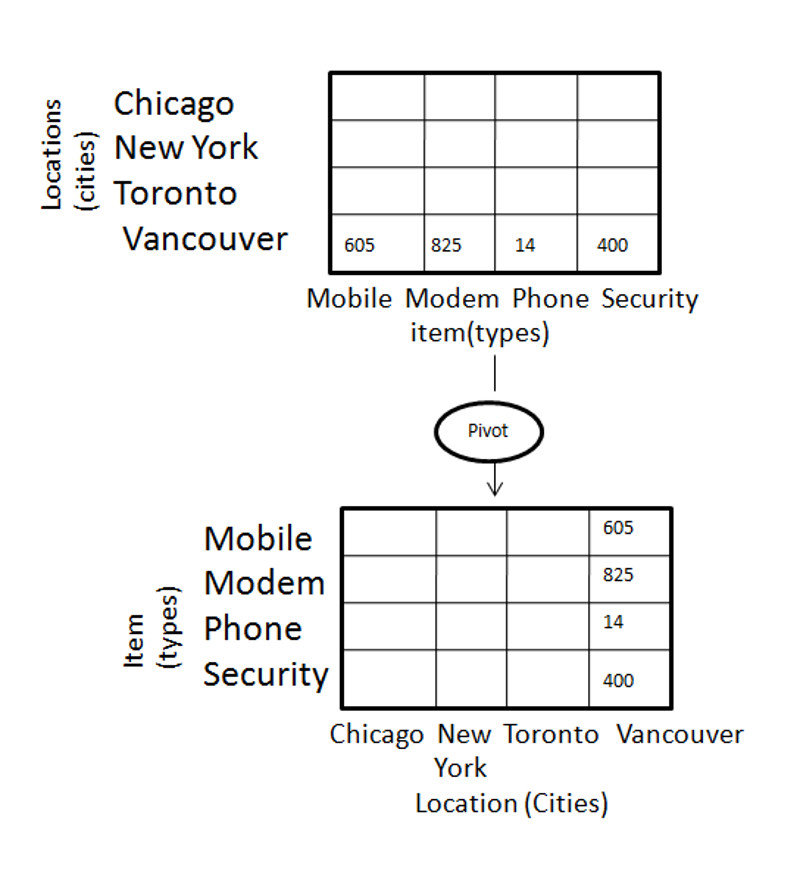
\includegraphics[scale=0.3]{pivot}
  \end{center}
}
\end{frame}


\end{document}
